% Created 2023-02-26 Sun 12:27
% Intended LaTeX compiler: pdflatex
\documentclass[11pt]{article}
\usepackage[utf8]{inputenc}
\usepackage[T1]{fontenc}
\usepackage{graphicx}
\usepackage{longtable}
\usepackage{wrapfig}
\usepackage{rotating}
\usepackage[normalem]{ulem}
\usepackage{amsmath}
\usepackage{amssymb}
\usepackage{capt-of}
\usepackage{hyperref}
\author{Yusheng Zhao}
\date{\today}
\title{Homework 1}
\hypersetup{
 pdfauthor={Yusheng Zhao},
 pdftitle={Homework 1},
 pdfkeywords={},
 pdfsubject={},
 pdfcreator={Emacs 28.2 (Org mode 9.6)}, 
 pdflang={English}}
\begin{document}

\maketitle
\tableofcontents


\section{Problem 1}
\label{sec:org9f5af3a}
\begin{itemize}
\item Name: SPERM WHALE MYOGLOBIN F46V N-BUTYL ISOCYANIDE AT PH 9.0
\item ID: 101M
\begin{figure}[htbp]
\centering
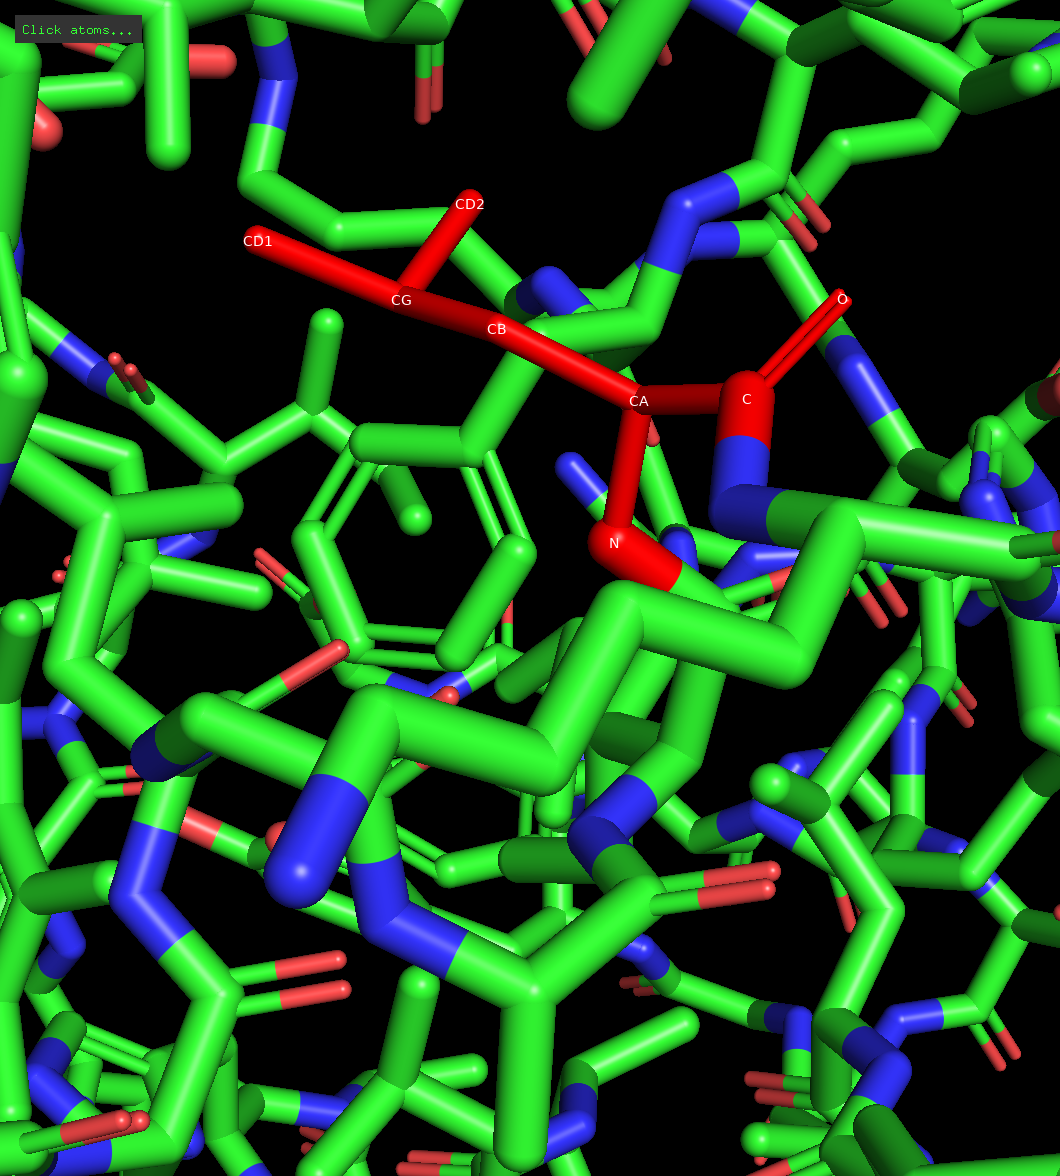
\includegraphics[width=.9\linewidth]{./sticks.png}
\caption{Illustration of molecule with sticks, atoms names of one amino acid labeled.}
\end{figure}

\begin{figure}[htbp]
\centering
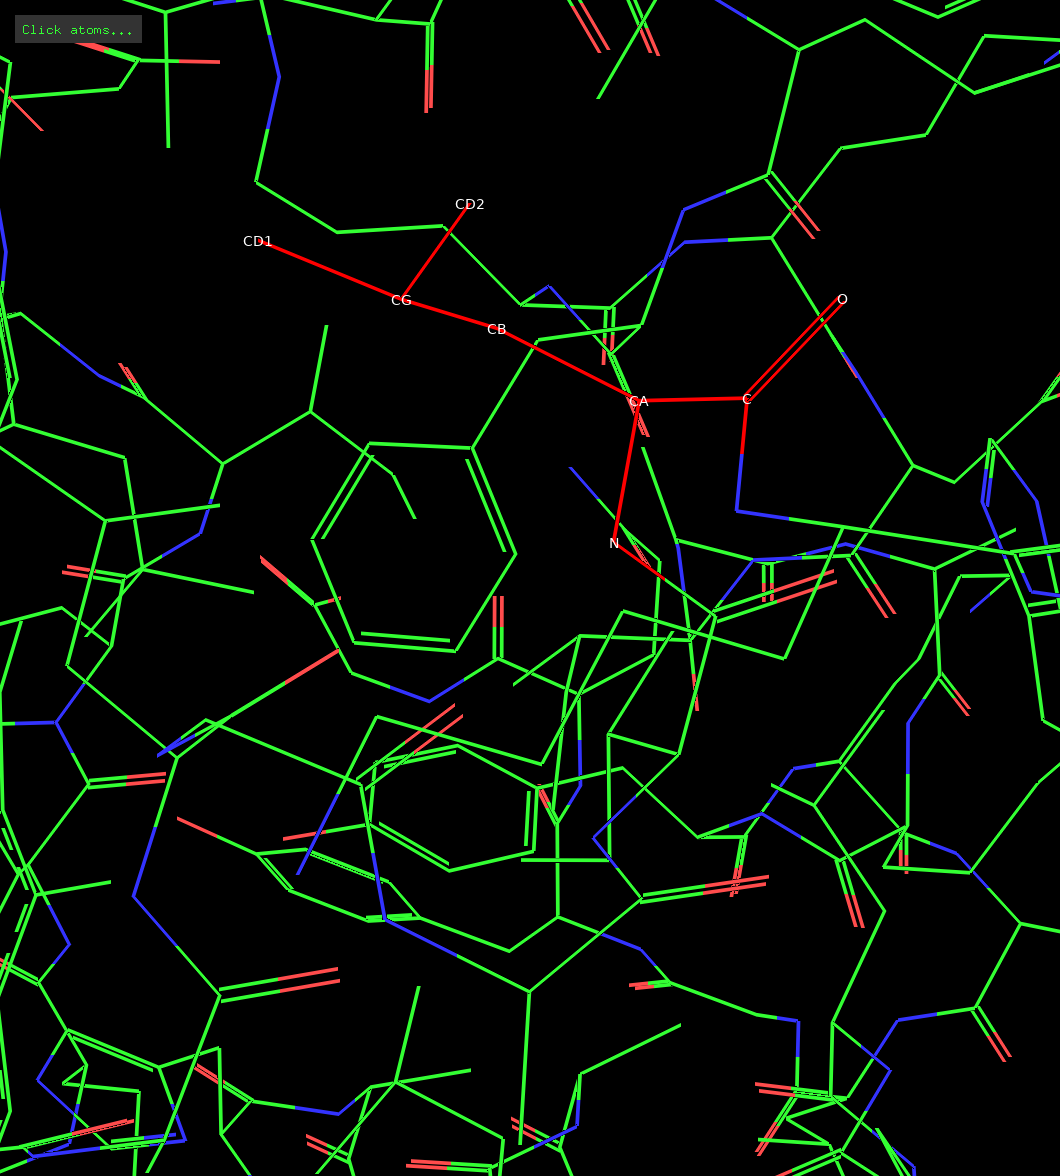
\includegraphics[width=.9\linewidth]{./lines.png}
\caption{Illustration of molecule with lines, atoms of one amino acid labelled}
\end{figure}

\begin{figure}[htbp]
\centering
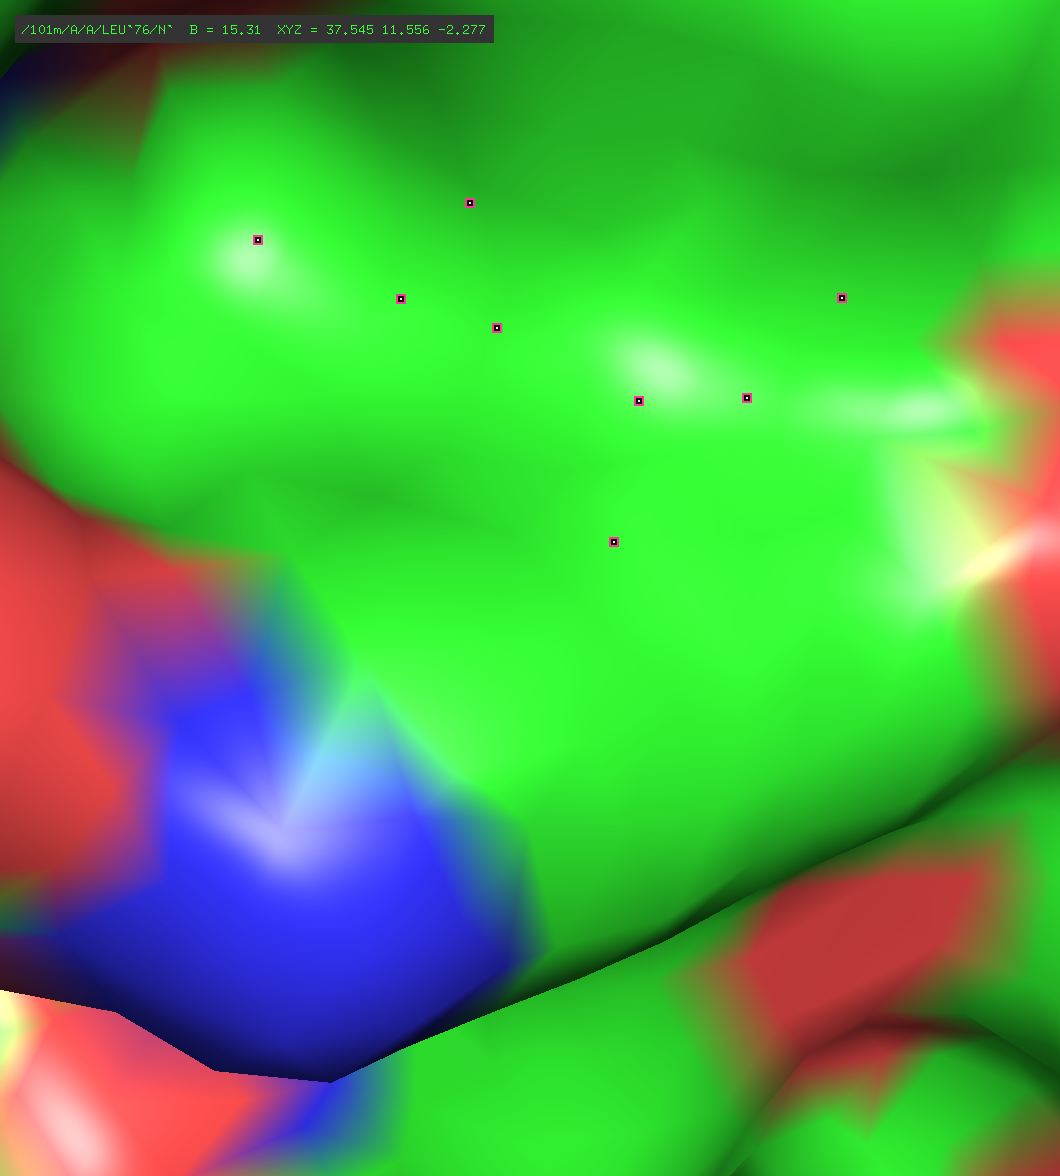
\includegraphics[width=.9\linewidth]{./surfaces.png}
\caption{Illustration of molecule with surfaces, atoms and names hidden under surface}
\end{figure}
\end{itemize}

\begin{figure}[htbp]
\centering
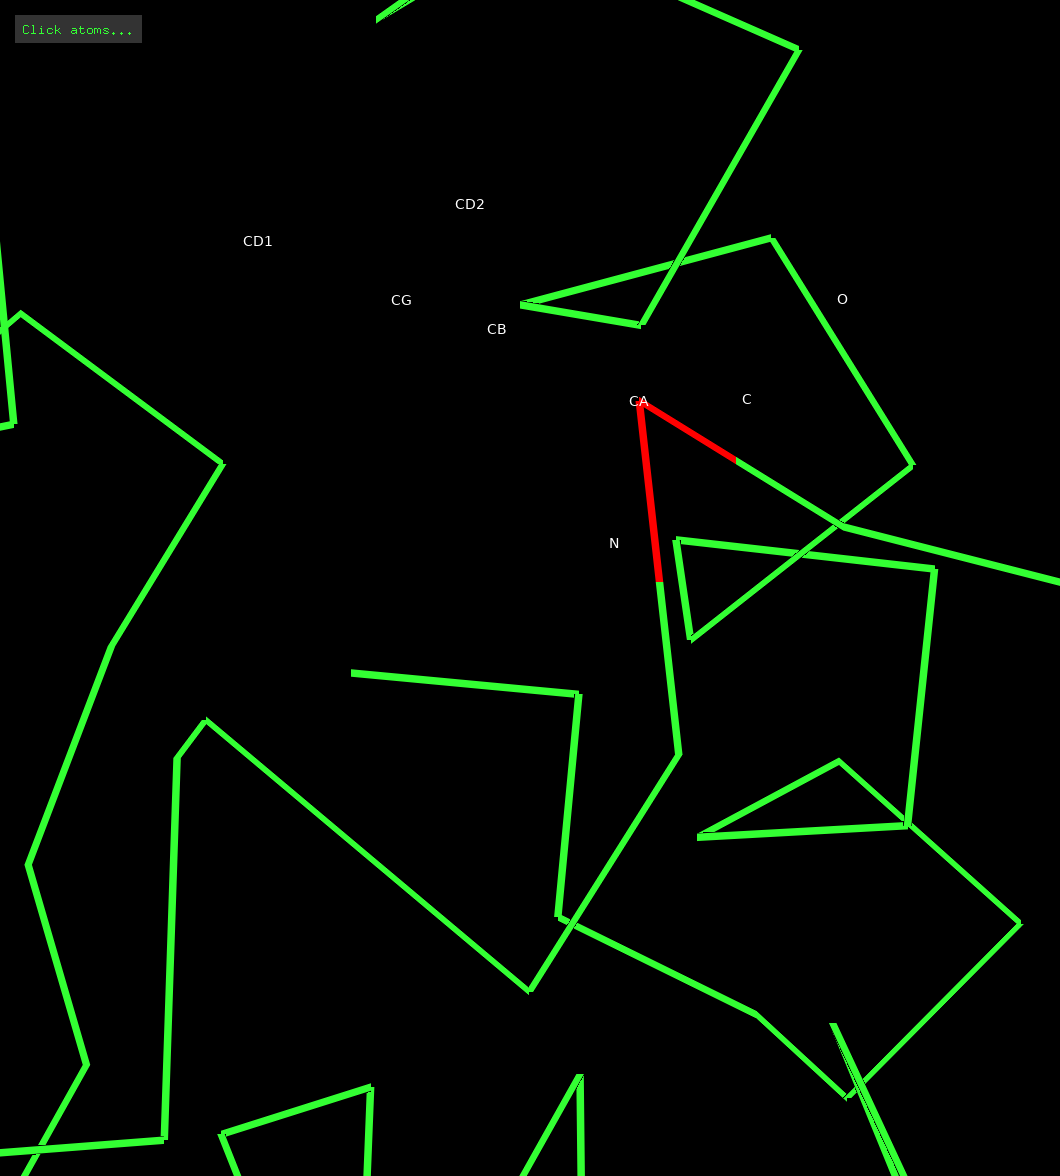
\includegraphics[width=.9\linewidth]{./ribbons.png}
\caption{Illustration of molecule with ribbons, atoms hidden but labels are in view.}
\end{figure}
\end{document}